% !TeX root = ../main.tex
\documentclass[./../main.tex]{subfiles}

\begin{document}

Phần mềm quản lý sắn KOICA được chia thành hai phần phát triển: frontend, và backend.

\section{Thiết kế kiến trúc}

Hệ thống sử dụng mô hình 3 lớp (Three-layer architecture). Mô hình 3 lớp phân chia các thành phần trong hệ thống theo nhóm chức năng, có nghĩa là các thành phần có cùng chức năng sẽ được nhóm lại với nhau để các công việc và dữ liệu trong từng nhóm không bị trùng lặp cũng như dễ dàng trao đổi giữa các thành phần đó.

\begin{figure}[H]
	\centering
	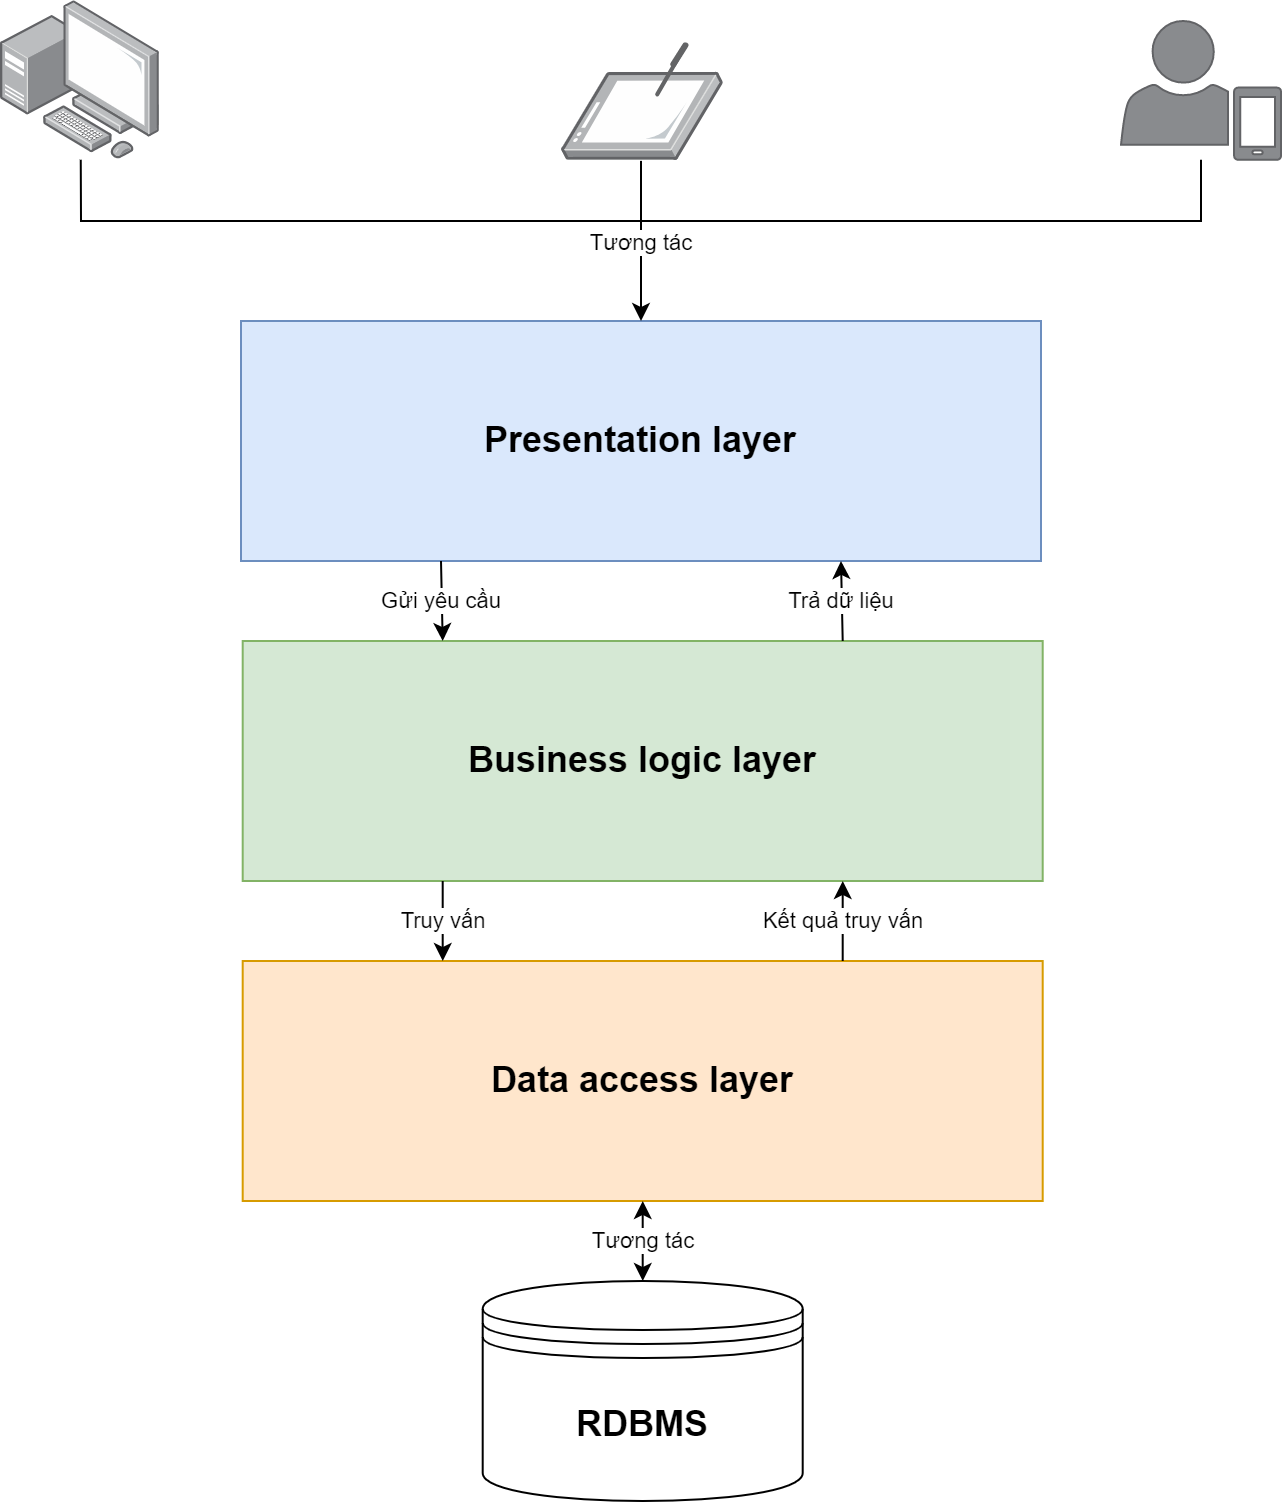
\includegraphics[width=\linewidth]{./img/architecture.png}
	\caption{Mô hình 3 lớp}
    \label{fig:architecture}
\end{figure}

Từ hình \ref{fig:architecture}, có thể diễn giải khái quát mô hình 3 lớp như sau:
\begin{itemize}
    \item \textbf{\textit{Presentation layer}} (Lớp trình bày): Sử dụng ReactJS và các thư viện hỗ trợ. Người dùng hệ thống (khách, người dùng, quản trị viên) sử dụng các thiết bị điện tử có kết nối mạng (máy tính cá nhân, máy tính bảng, điện thoại thông minh,...) tương tác với các thành phần được hiển thị trên giao diện thông qua lớp trình bày. Lớp này ngoài tiếp nhận các tương tác và gửi đi còn tiếp nhận dữ liệu từ lớp xử lý nghiệp vụ để hiển thị cho người sử dụng.
    \item \textbf{\textit{Business logic layer}} (Lớp xử lý nghiệp vụ): Sử dụng Directus. Sau khi tiếp nhận dữ liệu về các thao tác đã nhắc đến, lớp xử lý nghiệp vụ thực hiện việc phân tích dữ liệu và gửi truy vấn cơ sở dữ liệu đến lớp truy cập dữ liệu nếu cần rồi trả về dữ liệu đã được định dạng lại cho lớp trình bày.
    \item \textbf{\textit{Data access layer}} (Lớp truy cập dữ liệu): Sử dụng PostgreSQL được tích hợp trong Directus. Lớp này thực hiện các truy vấn dữ liệu như đầu vào và đầu ra là các kết quả sau khi truy vấn vào hệ quản trị cơ sở dữ liệu quan hệ.
\end{itemize}

\subsection{Lớp trình bày}
Lớp có hai thành phần chính sau đây với những chức năng cụ thể:
\begin{itemize}
    \item \acrshort{ui} Components gồm các thành phần tạo nên giao diện đồ họa người dùng (\acrshort{gui}). Chúng chịu trách nhiệm thu nhận và hiển thị dữ liệu.
    Ví dụ: bảng dữ liệu, các phím bấm, đường dẫn liên kết, ô nhập dữ liệu,...
    \item \acrshort{ui} Process Components là thành phần chịu trách nhiệm quản lý các quá trình chuyển đổi giữa các giao diện người dùng,...
    Ví dụ: hiển thị màn hình thông tin sắn, hiển thị màn hình thông tin chi tiết bệnh về sắn, hiển thị màn hình tra cứu dịch bệnh trên bản đồ,...
\end{itemize}

\subsection{Lớp xử lý nghiệp vụ}
Lớp này gồm 4 thành phần:
\begin{itemize}
    \item Service interface là thành phần giao diện cho các dịch vụ mà lớp này cung cấp cho lớp trình bày sử dụng. Trong hệ thống, hai lớp tương tác với nhau thông qua \acrshort{api}.
    \item Bussiness components chịu trách nhiệm kiểm tra các quy tắc nghiệp vụ, ràng buộc logic và thực hiện các công việc xử lý logic. Các thành phần này cũng xử lý các dịch vụ do service interface cung cấp mà business workflows sẽ sử dụng tới.
    \item Bussiness workflows chịu trách nhiệm xác định và điều phối các quy trình nghiệp vụ gồm nhiều bước và kéo dài. Những quy trình này phải được sắp xếp và thực hiện theo thứ tự chính xác giống như luồng hoạt động đã được đề ra trong phần phân tích.
    \item Bussiness entities thường được sử dụng như các đối tượng dữ liệu chuyển đổi giữa lớp này và lớp truy cập dữ liệu (DTO).
    Ví dụ: tạo 1 lớp sắn, gồm các trường id, label, name,... để phục vụ cho việc trao đổi với các hàm trong chính lớp này và cả các lớp khác,...
\end{itemize}

\subsection{Lớp truy cập dữ liệu}
Lớp truy cập dữ liệu bao gồm:
\begin{itemize}
    \item Data access logic components chịu trách nhiệm chính lưu trữ và truy xuất dữ liệu từ cơ sở dữ liệu của hệ thống, ngoài ra còn giúp cho việc cấu hình và bảo trì.
    \item Service agents gọi và tương tác với các dịch vụ từ bên ngoài một cách dễ dàng và đơn giản.
    \item Directus ngoài việc có thể tạo cơ sở dữ liệu một cách trực quan, thì việc tương tác với cơ sở dữ liệu (lưu trữ, truy xuất dữ liệu) đã được tích hợp sẵn. Thêm vào đó, một số tiện ích bổ sung để kết nối với các dịch vụ bên ngoài cũng bao gồm trong công cụ này; phần công việc gửi thư điện tử tự động chứa token đổi mật khẩu trong ca sử dụng quên mật khẩu đã sử dụng \acrshort{smtp} của của Directus.
\end{itemize}

\section{Thiết kế các sơ đồ hệ thống}
\subsection{Cơ sở dữ liệu}
\begin{figure}[H]
	\centering
	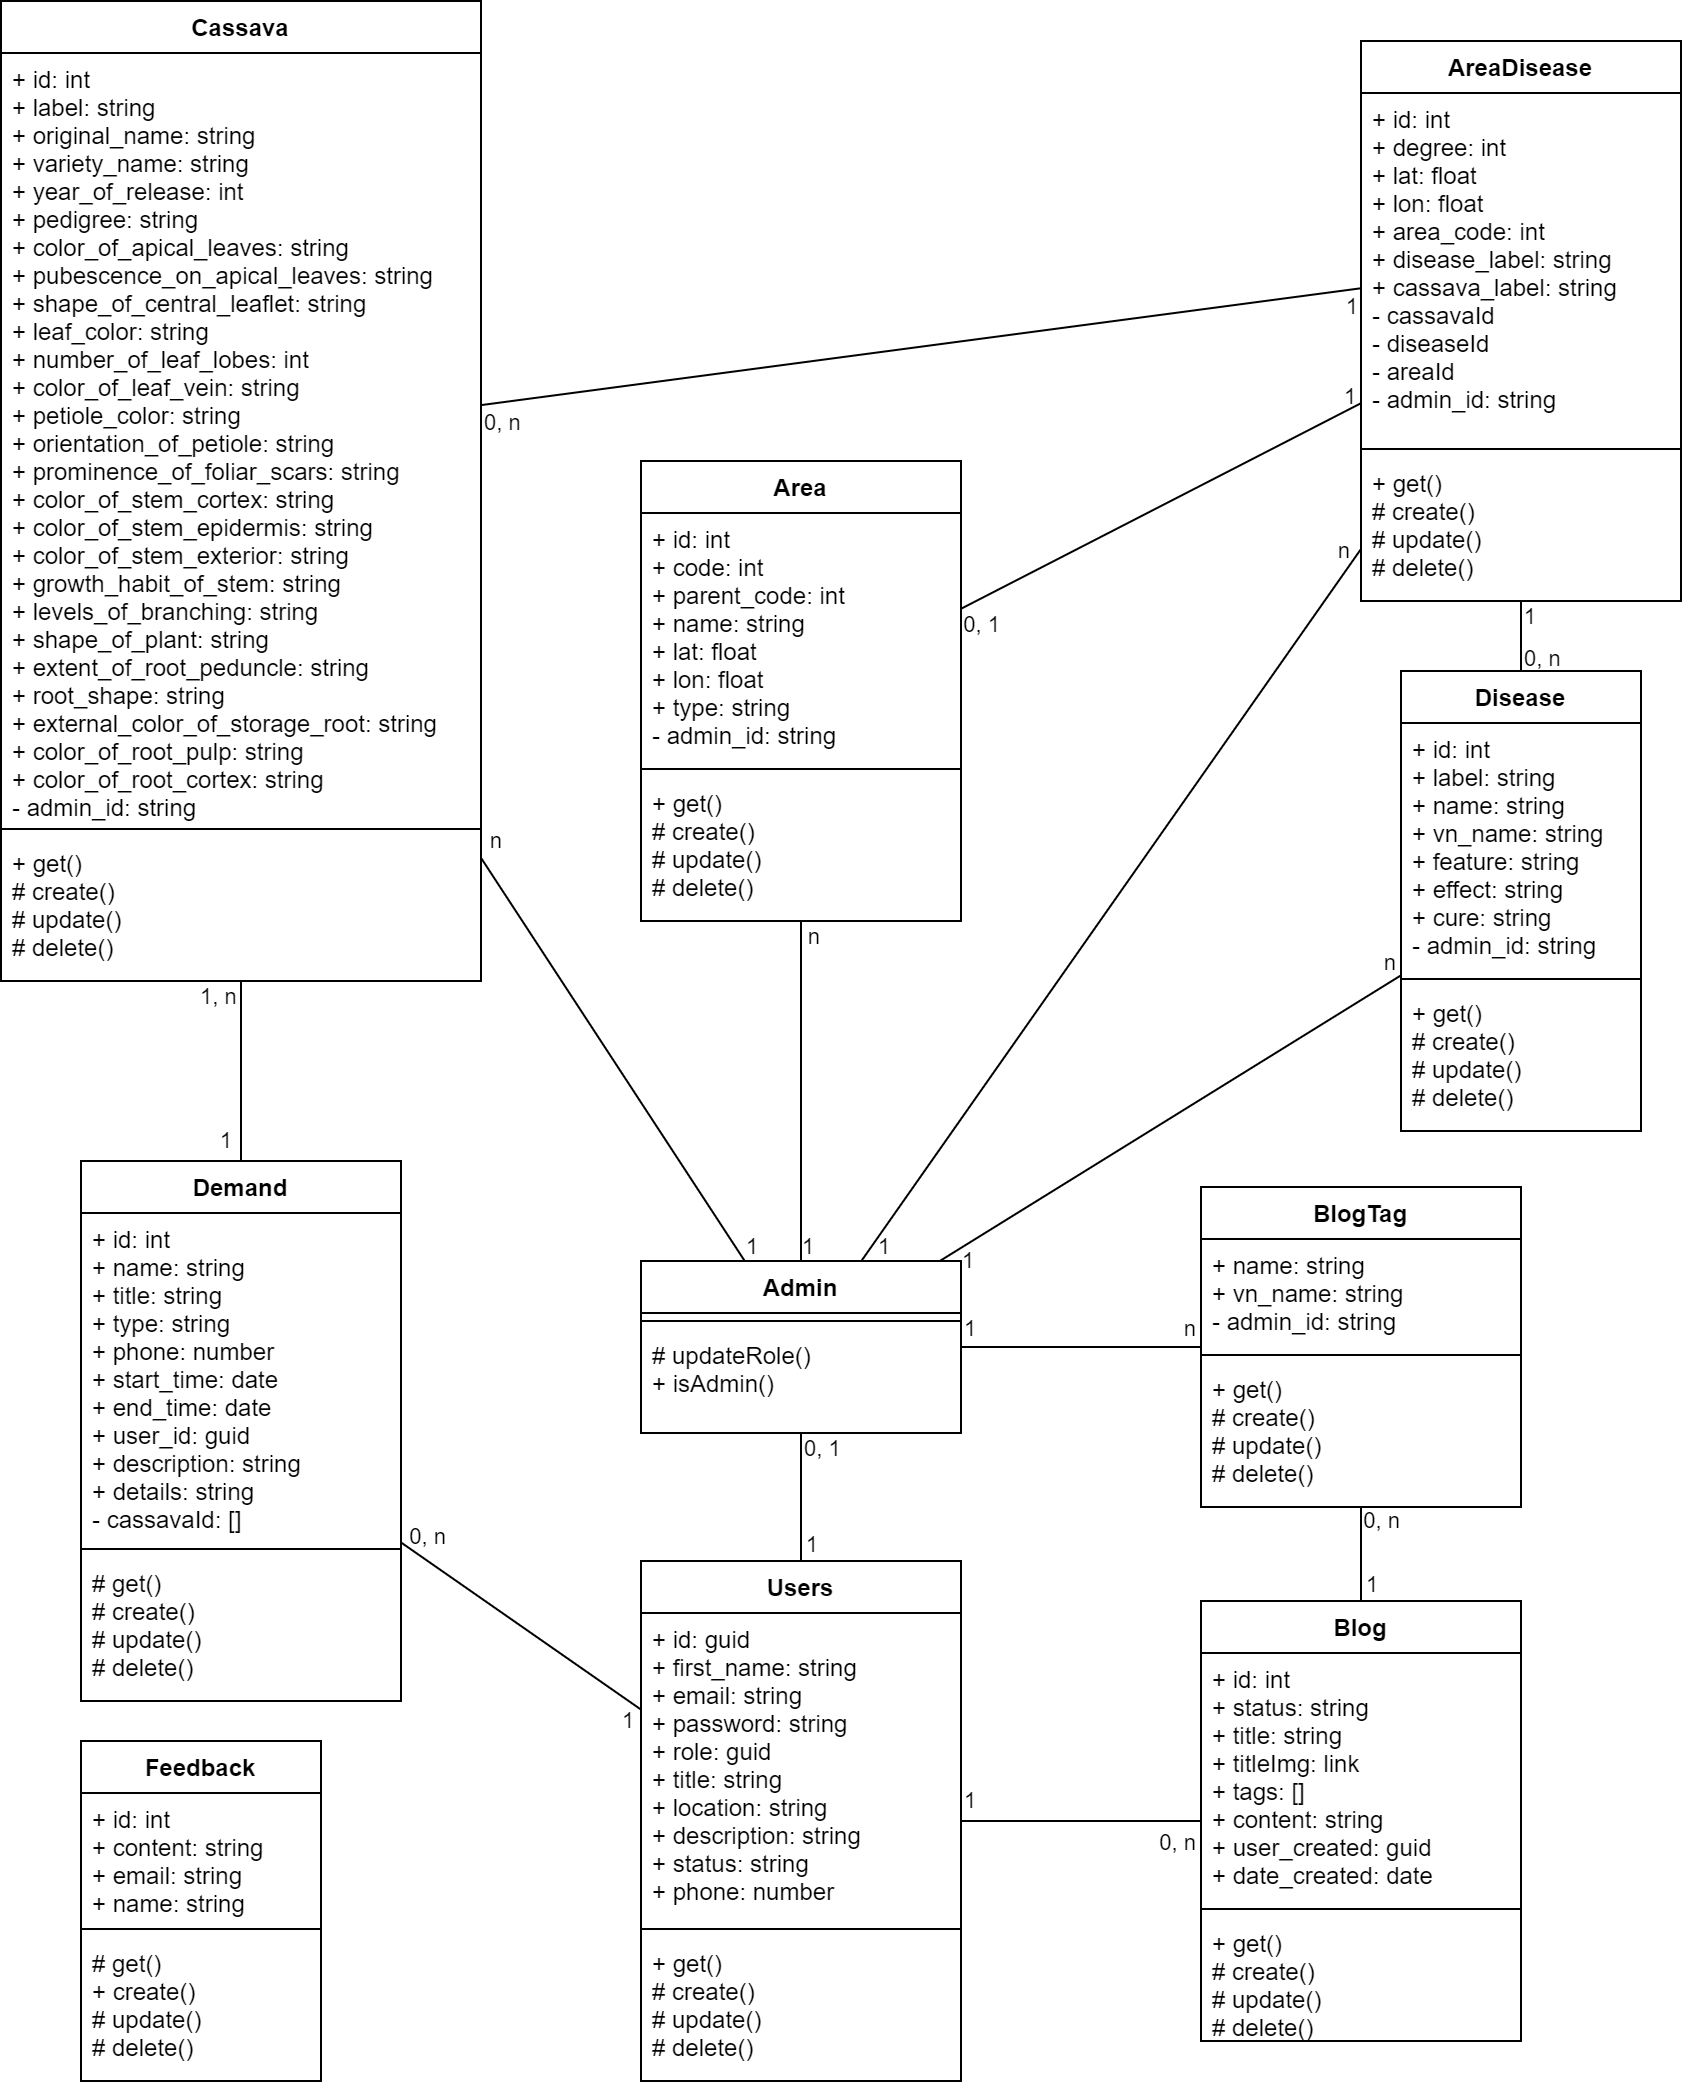
\includegraphics[width=0.9\linewidth]{./img/db.png}
    \caption{Sơ đồ cơ sở dữ liệu}
\end{figure}
Từ các đặc tả ca sử dụng, xác định được luồng hoạt động của hệ thống và mối quan hệ giữa các lớp, cơ sở dữ liệu được thiết kế với các bảng tương ứng với các lớp thực thể (Entity classes) như hình trên. Có thể coi các trường dữ liệu mà lớp thực thể chứa được ánh xạ từ các bảng trong cơ sở dữ liệu của hệ thống. Các trường thông tin công khai được hiển thị trong sơ đồ để người dùng có thể nắm bắt nội dung, tuy nhiên để tác động, thay đổi nó thì cần phải có quyền tùy theo đối tượng dùng là ai. Sơ đồ còn thể hiện mối liên kết giữa các đối tượng. Cụ thể như sau:
\begin{itemize}
    \item Giữa Cassava và AreaDisease, giữa Disease và AreaDisease, giữa Area và AreaDisease đều có mối quan hệ 1 - n. Có nghĩa là, với 1 dịch bệnh đang diễn ra sẽ gắn với 1 giống sắn đang mắc 1 loại bệnh tại 1 khu vực cụ thể ở tỉnh Tây Ninh, có thể là cấp quận, huyện hoặc phường, xã hoặc một vị trí cụ thể khác và một giống sắn có thể mắc nhiều loại bệnh, một bệnh cũng có thể xảy ra trên nhiều giống sắn, một khu vực có thể có nhiều dịch bệnh đang diễn ra. Tuy nhiên không phải giống sắn nào cũng mắc bệnh, không phải ở khu vực nào cũng diễn ra dịch bệnh, có thể hiểu là, mối quan hệ này sẽ không bắt buộc ở phía Cassava, Disease, Area.
    \item Giữa Admin và các đối tượng: Cassava, AreaDisease, Area, Disease, BlogTag, là mối quan hệ 1 - n. Có nghĩa là, mỗi quản trị viên sẽ liên kết tới các dòng dữ liệu mà người đó tạo ra, Khi quản trị viên khác cập nhật lại dữ liệu thì liên kết tới dòng dữ liệu đó sẽ do quản trị viên vừa thực hiện thay đổi chịu trách nhiệm.
    \item Giữa Admin và Users có mối quan hệ 1 - 1. Có nghĩa là với 1 quản trị viên sẽ tương ứng với 1 người dùng nhưng có nhiều quyền hạn hơn. Tuy nhiên, không phải người dùng nào cũng là quản trị viên, vậy nên mối quan hệ này ở phía quản trị viên là không bắt buộc.
    \item Giữa Demand và Cassava là mối quan hệ 1 - n. Có nghĩa là với 1 đề xuất trao đổi sắn sẽ có thể có ít nhất một hay nhiều loại sắn được thêm vào đề xuất.\\ Giữa Users và Demand là mối quan hệ 1 - n. Có nghĩa là 1 người dùng có thể tạo nhiều đề xuất hoặc không có đề xuất nào nếu người dùng không có nhu cầu. Quản trị viên cũng được thừa hưởng điều này từ người dùng.
    \item Giữa Blog và BlogTag là mối quan hệ 1 - n. Có nghĩa là 1 bài viết trên diễn đàn có thể có nhiều hơn một thẻ tag liên quan đến nội dung bài viết hoặc không có thẻ tag nào.\\
    Giữa Users và Blog là mối quan hệ 1 - n. Có nghĩa là mỗi người dùng có thể viết một hoặc nhiều bài viết hoặc cũng có thể không có bài viết nào. Vậy nên mối quan hệ này là không bắt buộc ở phía người dùng. Quản trị viên cũng được thừa hưởng điều này từ người dùng.
\end{itemize}

\subsection{Các lớp điều khiển}
\begin{figure}[H]
	\centering
	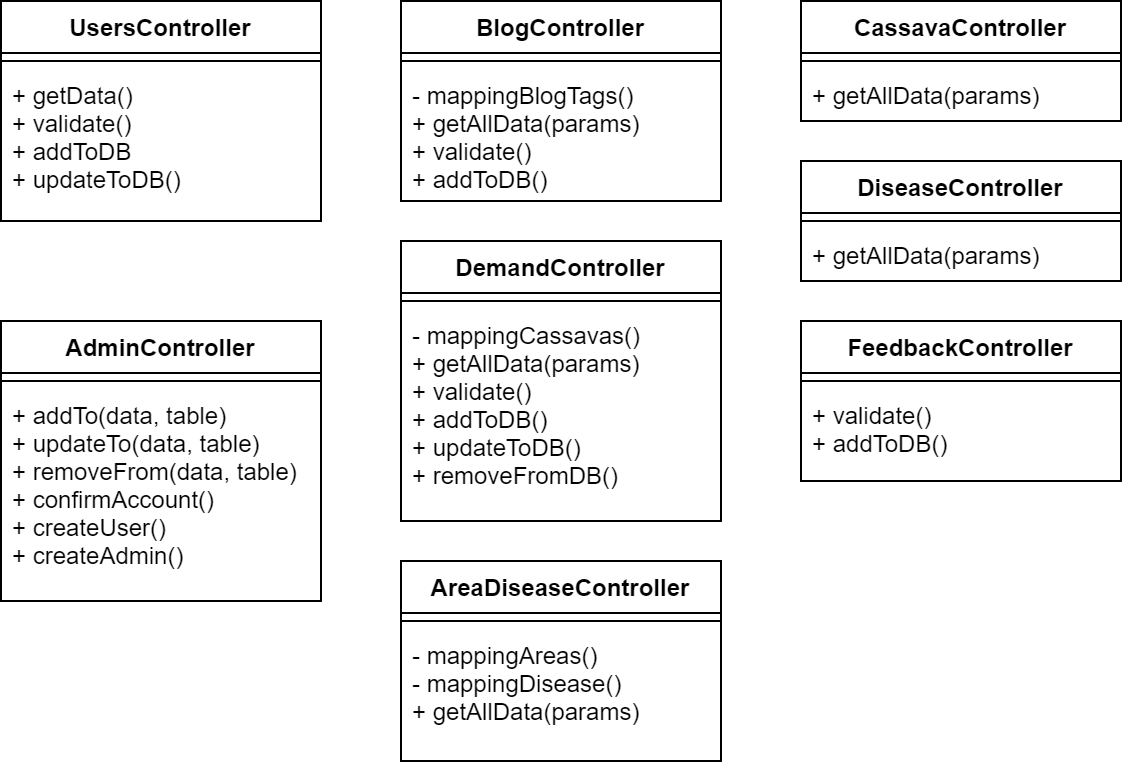
\includegraphics[width=\linewidth]{./img/controller.png}
	\caption{Sơ đồ các lớp điều khiển}
\end{figure}
Các lớp điều khiển (Control classes) được thiết kế để phục vụ cho việc truy xuất, xử lý và cập nhật dữ liệu trong cơ sở dữ liệu. Vì Directus là Headless \acrshort{cms} nên hầu như việc xử lý dữ liệu sẽ được thực hiện ở phía frontend thay vì backend như các hệ thống thông thường. Sau khi xử lý các logic để chuẩn hóa thông tin, phía frontend sẽ gửi các yêu cầu truy vấn để lấy dữ liệu theo các biến truyền đi, với các yêu cầu thêm mới dữ liệu vào cơ sở dữ liệu hoặc sửa đổi dữ liệu đã tồn tại, thông tin sẽ được gửi dưới dạng biểu mẫu đã được chỉnh đúng định dạng. Directus nhận được yêu cầu sẽ thực hiện nhiệm vụ tương ứng và trả lại kết quả hoặc cập nhật cơ sở dữ liệu rồi trả lại kết quả cho người dùng về kết quả nhiệm vụ thành công hay không. 

\subsection{Các lớp giao diện}
\begin{figure}[H]
	\centering
	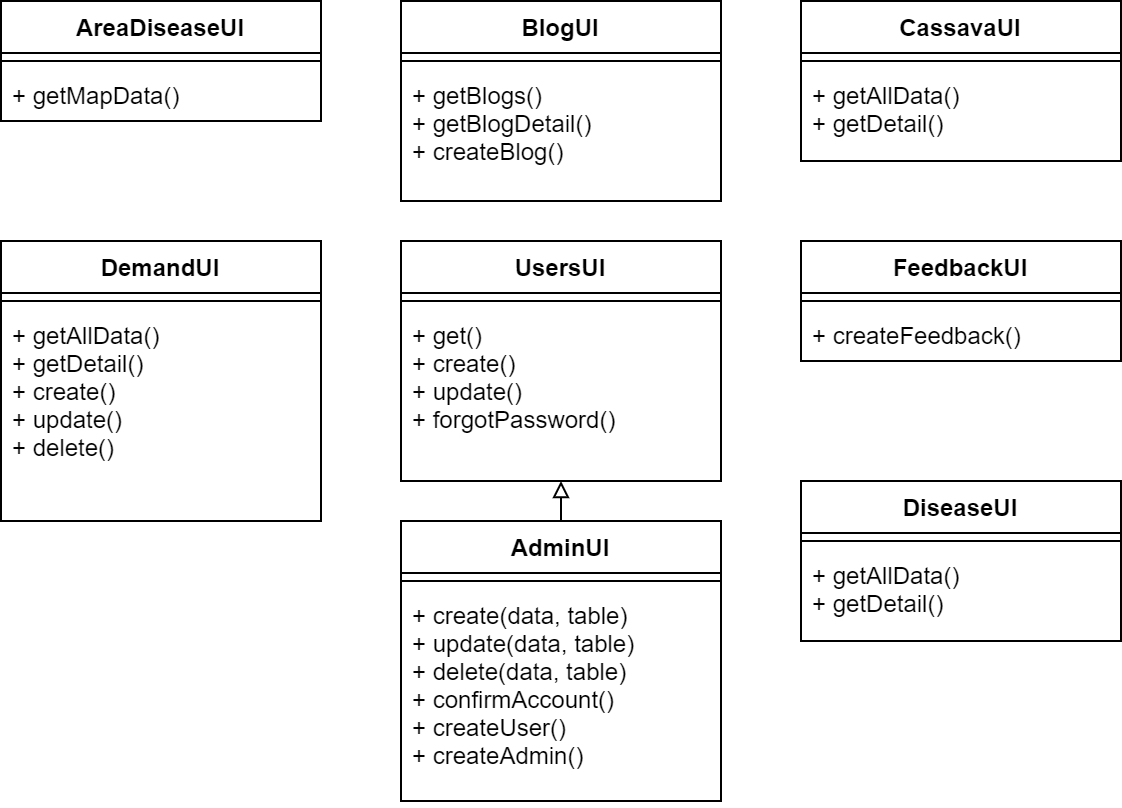
\includegraphics[width=\linewidth]{./img/boundary.png}
	\caption{Sơ đồ các lớp giao diện}
\end{figure}
Các lớp giao diện (Boundary classes), hay còn gọi là lớp sẽ hiển thị giao diện để người dùng tương tác với hệ thống. Thông qua giao diện, các tác nhân có thể thực hiện các chức năng theo quyền hạn tương ứng. Ở các lớp này, dữ liệu sẽ cần phải được chuẩn hóa theo đúng định dạng để đảm bảo việc hiển thị thông tin được chuẩn xác nhất, đảm bảo trải nghiệm người dùng. Nó bao gồm các bảng dữ liệu về sắn, bản đồ dịch bệnh đang diễn ra tại tỉnh Tây Ninh, các biểu mẫu đăng ký, tạo bài viết mới, sửa thông tin cá nhân, thêm mới đề xuất, các nút bấm để xác nhận, gửi yêu cầu đi,... dùng để hiển thị cho người dùng và thông qua đó gửi yêu cầu thực hiện các nhiệm vụ đến lớp điều khiển. Ở phía frontend, khi gửi biểu mẫu cần phải kiểm tra xem các trường thông tin đã đúng định dạng chưa trước khi gửi cho phía backend.


\section{Thiết kế Backend}
\subsection{Cấu trúc thư mục}
Các tệp và thư mục được sắp xếp như sau:
\begin{itemize}
    \item \textbf{/csv}: Chứa các tệp định dạng .csv, có dữ liệu có thể sử dụng để tải lên dữ liệu mặc định cho hệ thống.
    \item \textbf{/data}: Được Directus tự động tạo ra dùng để lưu trữ dữ liệu vào cơ sở dữ liệu PostgreSQL.
    \item \textbf{/node\_modules}: Được \acrshort{npm}  tạo ra, chứa các thư mục và tệp các dòng lệnh của framework hay thư viện dùng trong hệ thống.
    \item \textbf{/uploads}: Chứa các tệp ảnh được tải lên hệ thống.
    \item \textbf{.env}: Là tệp dữ liệu các biến môi trường được Directus sử dụng để cài đặt hệ thống theo nhu cầu lập trình viên.
    \item \textbf{.env.example}: Tệp ví dụ các biến môi trường.
    \item \textbf{.gitignore}: Quản lý các thư mục, tệp trong git.
    \item \textbf{docker-compose.yml}: Khai báo các container cần thiết để chạy hệ thống thông qua docker.
    \item \textbf{init.sh}: Tệp chứa các câu lệnh khi khởi tạo hệ thống trong docker container.
    \item \textbf{package-lock.json}: Tệp được tạo ra một cách tự động chứa dữ liệu liên quan tương ứng với package.json.
    \item \textbf{package.json}: Chứa thông tin tổng quan về phần backend, các framework, thư viện và phiên bản được sử dụng.
    \item \textbf{README.md}: Là bản hướng dẫn khi cài đặt, sửa lỗi hệ thống.
    \item \textbf{schema.yaml}: Được Directus tạo ra khi tạo cơ sở dữ liệu và lưu thông tin về cấu trúc cơ sở dữ liệu.
\end{itemize}

\subsection{Thiết kế \acrshort{api}}
Các \acrshort{api}  được sử dụng hầu như đều có cấu trúc dạng: [action\_name] \url{[base_url]/items/[db_name]?[params]} và một số \acrshort{api}  có dạng khác.
Trong đó:
\begin{itemize}
    \item "action\_name" là tên hành động tác động tới cơ sở dữ liệu.\\ Các tên hành động có thể sử dụng bao gồm: get (lấy dữ liệu), post (gửi dữ liệu), patch (cập nhật dữ liệu).
    \item "base\_url" là đường dẫn gốc tới phía backend.\\ Nếu tự chạy cả backend và frontend thì biến này sẽ có giá trị mặc định là http://localhost:8005.  
    \item "db\_name" là tên bảng dữ liệu được truy vấn tới.\\ Các bảng dữ liệu có trong hệ thống gồm: area, area\_disease, blog, blog\_tag, cassava, cassava\_files, demand, diagnostics, diagnostics\_files, disease, disease\_files, feedback.
    \item "params" là các cặp tham số theo kiểu (key: value) có thể hiểu như (tên tham số: giá trị tham số) được truyền cho backend, phục vụ cho việc truy vấn cơ sở dữ liệu có điều kiện.\\ Các cặp (tên tham số - dạng dữ liệu giá trị tham số) được sử dụng:
    \begin{itemize}
        \item{[fields - string]: trả về dữ liệu của các cột trong bảng, nếu giá trị = * thì trả về các trường có trong bảng, nếu giá trị bằng [tên trường].[tên trường con] thì trả về các trường con trong trường dữ liệu tương ứng.}
        \item{[limit - int]: giới hạn số dữ liệu trả về, nếu giá trị = -1 thì trả về tất cả các dòng dữ liệu.}
        \item{[aggregate[count] - string]: đếm các hàng dữ liệu theo truy vấn cột tương ứng với giá trị truyền vào, nếu giá trị = * thì trả về tổng số hàng trong bảng.}
        \item{[filter[tên trường][\_eq] - string]: lọc dữ liệu theo trường dữ liệu tương ứng có giá trị bằng giá trị truyền lên.}
    \end{itemize}
\end{itemize}

Bảng dưới đây sẽ liệt kê các \acrshort{api}  được dùng trong hệ thống để frontend tương tác với backend:
\begin{longtable}{| p{0.07\linewidth} | p{0.2\linewidth} | p{0.3\linewidth} | p{0.3\linewidth} |}
\caption{\label{table-api}Bảng tổng hợp \acrshort{api} } \label{list-api }
\hline
\textbf{STT} & \textbf{Phương thức} & \textbf{URL} & \textbf{Mô tả} \\ \hline 
\centerline{1} & GET & \url{/items/blog_tag?limit=-1} & Lấy các thẻ tag bài viết. \\ \hline
\centerline{2} & GET & \url{/items/blog?aggregate[count]=*} & Lấy số lượng các bài viết có trên hệ thống. \\ \hline
\centerline{3} & GET & \url{/items/blog?limit=-1} & Lấy các bài viết. \\ \hline
\centerline{4} & GET & \url{/items/blog/?fields=*&filter[id][_eq]=id} & Lấy chi tiết bài viết theo id. \\ \hline
\centerline{5} & POST & \url{/items/blog} & Tạo bài viết mới. \\ \hline
\centerline{6} & GET & \url{/items/cassava?fields=*} & Lấy thông tin về các loại sắn. \\ \hline
\centerline{7} & GET & \url{/items/cassava?fields=*,images.*&filter[id][_eq]=id} & Lấy chi tiết thông tin loại sắn theo id. \\ \hline
\centerline{8} & POST & \url{/items/diagnostics} & Tạo tệp ảnh chẩn đoán mới. \\ \hline
\centerline{9} & GET & \url{/items/disease?fields=*} & Lấy thông tin các bệnh trên cây sắn. \\ \hline
\centerline{10} & GET & \url{/items/disease?fields=*,images.*&filter[id][_eq]=id} & Lấy chi tiết thông tin bệnh trên cây sắn theo id. \\ \hline
\centerline{11} & POST & \url{/items/feedback} & Tạo nhận xét mới. \\ \hline
\centerline{12} & POST & \url{/files} & Tạo tệp ảnh mới và lưu vào cơ sở dữ liệu. \\ \hline
\centerline{13} & GET & \url{/items/area?limit=-1&filter[type][_eq]=type&filter[parent_code][_eq]=parent_code} & Lấy thông tin các khu vực ở tỉnh Tây Ninh theo type và parent\_code. \\ \hline
\centerline{14} & GET & \url{/items/area_disease?limit=-1} & Lấy thông tin các dịch bệnh. \\ \hline
\centerline{15} & GET & \url{/items/demand?filter[type][_eq]=type} & Lấy các đề xuất theo type = buy, type = sell. \\ \hline
\centerline{16} & POST & \url{/items/demand/id} & Lấy thông tin đề xuất cá nhân. \\ \hline
\centerline{17} & PATCH & \url{/items/demand/id} & Tạo đề xuất cá nhân mới. \\ \hline
\centerline{18} & DELETE & \url{/items/demand/id} & Sửa đề xuất cá nhân. \\ \hline
\centerline{19} & GET & \url{/items/demand?filter[type][_eq]=type&filter[user_id][_eq]=user_id} & Lấy thông tin đề xuất theo type và user\_id. \\ \hline
\centerline{20} & GET & \url{/users} & Lấy thông tin các nguồn cung. \\ \hline
\centerline{21} & GET & \url{/users/me} & Lấy thông tin người dùng hiện tại. \\ \hline
\centerline{22} & PATCH & \url{/users/me} & Sửa thông tin người dùng hiện tại. \\ \hline
\centerline{23} & POST & \url{/users} & Tạo yêu cầu đăng ký tài khoản. \\ \hline
\centerline{24} & POST & \url{/auth/password/request} & Tạo yêu cầu cấp lại mật khẩu. \\ \hline
\centerline{25} & POST & \url{/auth/password/reset} & Tạo yêu cầu đổi mật khẩu. \\ \hline
\centerline{26} & POST & \url{/auth/login} & Đăng nhập vào hệ thống. \\ \hline
\centerline{27} & POST & \url{auth/logout} & Đăng xuất khỏi hệ thống. \\ \hline
\centerline{28} & POST & \url{http://iai.uet.vnu.edu.vn:8001/classify_image} & Tạo yêu cầu chẩn đoán bằng ảnh. \\ \hline
\end{longtable}

\section{Thiết kế Frontend}
\subsection{Cấu trúc thư mục}
\begin{itemize}
    \item \textbf{/.nginx}: Cấu hình để tạo nên web server chạy trong docker.
    \item \textbf{/node\_modules}: Được \acrshort{npm}  tạo ra, chứa các thư mục và tệp các dòng lệnh của framework hay thư viện dùng trong hệ thống.
    \item \textbf{/public}: Chứa các tệp, các ảnh, logo dùng trong ứng dụng.
    \item \textbf{/src}: Bao gồm toàn bộ các tệp chứa mã lệnh thực thi chương trình và các tệp css để tạo nên giao diện cho trang web.
    \begin{itemize}
        \item \textbf{/components}: Gồm các thành phần có thể tái sử dụng trong hệ thống.
        \item \textbf{/helpers}: Chứa các hàm dùng chung cho cả việc lập trình giao diện.
        \item \textbf{/images}: Chứa các ảnh, các tệp .svg dùng trong giao diện.
        \item \textbf{/pages}: Gồm các trang có trong hệ thống.
        \item \textbf{/services}: Gồm các tệp xử lý việc gọi \acrshort{api}, các logic tính toán trong hệ thống, các hàm hỗ trợ cho việc tính toán, lưu trữ dữ liệu.
        \item \textbf{/styles}: Các tệp giúp cải thiện giao diện.
        \item \textbf{App.js}: Là trang chính, có nhiệm vụ điều hướng, khởi tạo các trang nhánh.
        \item \textbf{ComponentRenderer.js}: Giúp các trang có thêm hiệu ứng mặc định.
        \item \textbf{index.css}: Định dạng các thành phần trên giao diện cho index.js.
        \item \textbf{index.js}: Khởi tạo ứng dụng ReactJS.
        \item \textbf{style.css}: Định dạng các thành phần trên giao diện cho App.js.
        \item \textbf{tailwind.config.js}: Tệp cấu hình cho thư viện giao diện tailwind.
    \end{itemize}
    \item \textbf{.dockerignore}: Quản lý các thư mục, tệp trong docker.
    \item \textbf{.env}: Là tệp dữ liệu các biến môi trường sử dụng để cài đặt hệ thống theo nhu cầu lập trình viên.
    \item \textbf{.env.example}: Tệp ví dụ các biến môi trường.
    \item \textbf{.gitignore}: Quản lý các thư mục, tệp trong git.
    \item \textbf{babel-plugin-macro.config.js}: Giúp hệ thống vẽ các giao diện giữa các thư viện hỗ trợ về giao diện được sử dụng trong lập trình bằng JavaScript mà không yêu cầu người dùng cài thêm plugin babel khác.
    \item \textbf{carco.config.js}: Tệp giúp tạo lớp cấu hình cho ứng dụng ReactJs một cách dễ dàng và dễ hiểu.
    \item \textbf{docker-compose.yml}: Khai báo các container cần thiết để chạy hệ thống thông qua docker.
    \item \textbf{Dockerfile}: Giúp tạo container bằng docker.
    \item \textbf{jsconfig.json}: Cấu hình cho chương trình viết bằng JavaScript.
    \item \textbf{package-lock.json}: Tệp được tạo ra một cách tự động chứa dữ liệu liên quan tương ứng với package.json.
    \item \textbf{package.json}: Chứa thông tin tổng quan về các gói, các framework, thư viện và phiên bản được sử dụng.
    \item \textbf{postcss.config.js}: Tệp cấu hình cho thư viện giao diện tailwind với các tệp css.
    \item \textbf{README.md}: Là bản hướng dẫn khi cài đặt, sửa lỗi hệ thống.
    \item \textbf{yarn.lock}: Tương tự như package-lock.json nhưng được tạo bởi yarn.
\end{itemize}

\subsection{Thiết kế giao diện}
Khi thiết kế giao diện cần chú ý tới bố cục, màu sắc chủ đề và đảm bảo sự nhất quán giữa các thành phần trong trang. Từ các bản thiết kế giao diện, hệ thống sử dụng framework ReactJS và các thư viện hỗ trợ để đưa thiết kế lên trang web và hiển thị giao diện có khả năng tương tác. Vì người dùng có thể sử dụng phần mềm trên nhiều thiết bị nên cũng cần thiết kế giao diện phù hợp với từng kích thước khung khác nhau, đảm bảo tính linh hoạt. Dưới đây là một số thiết kế giao diện:

\begin{figure}[H]
\centering
    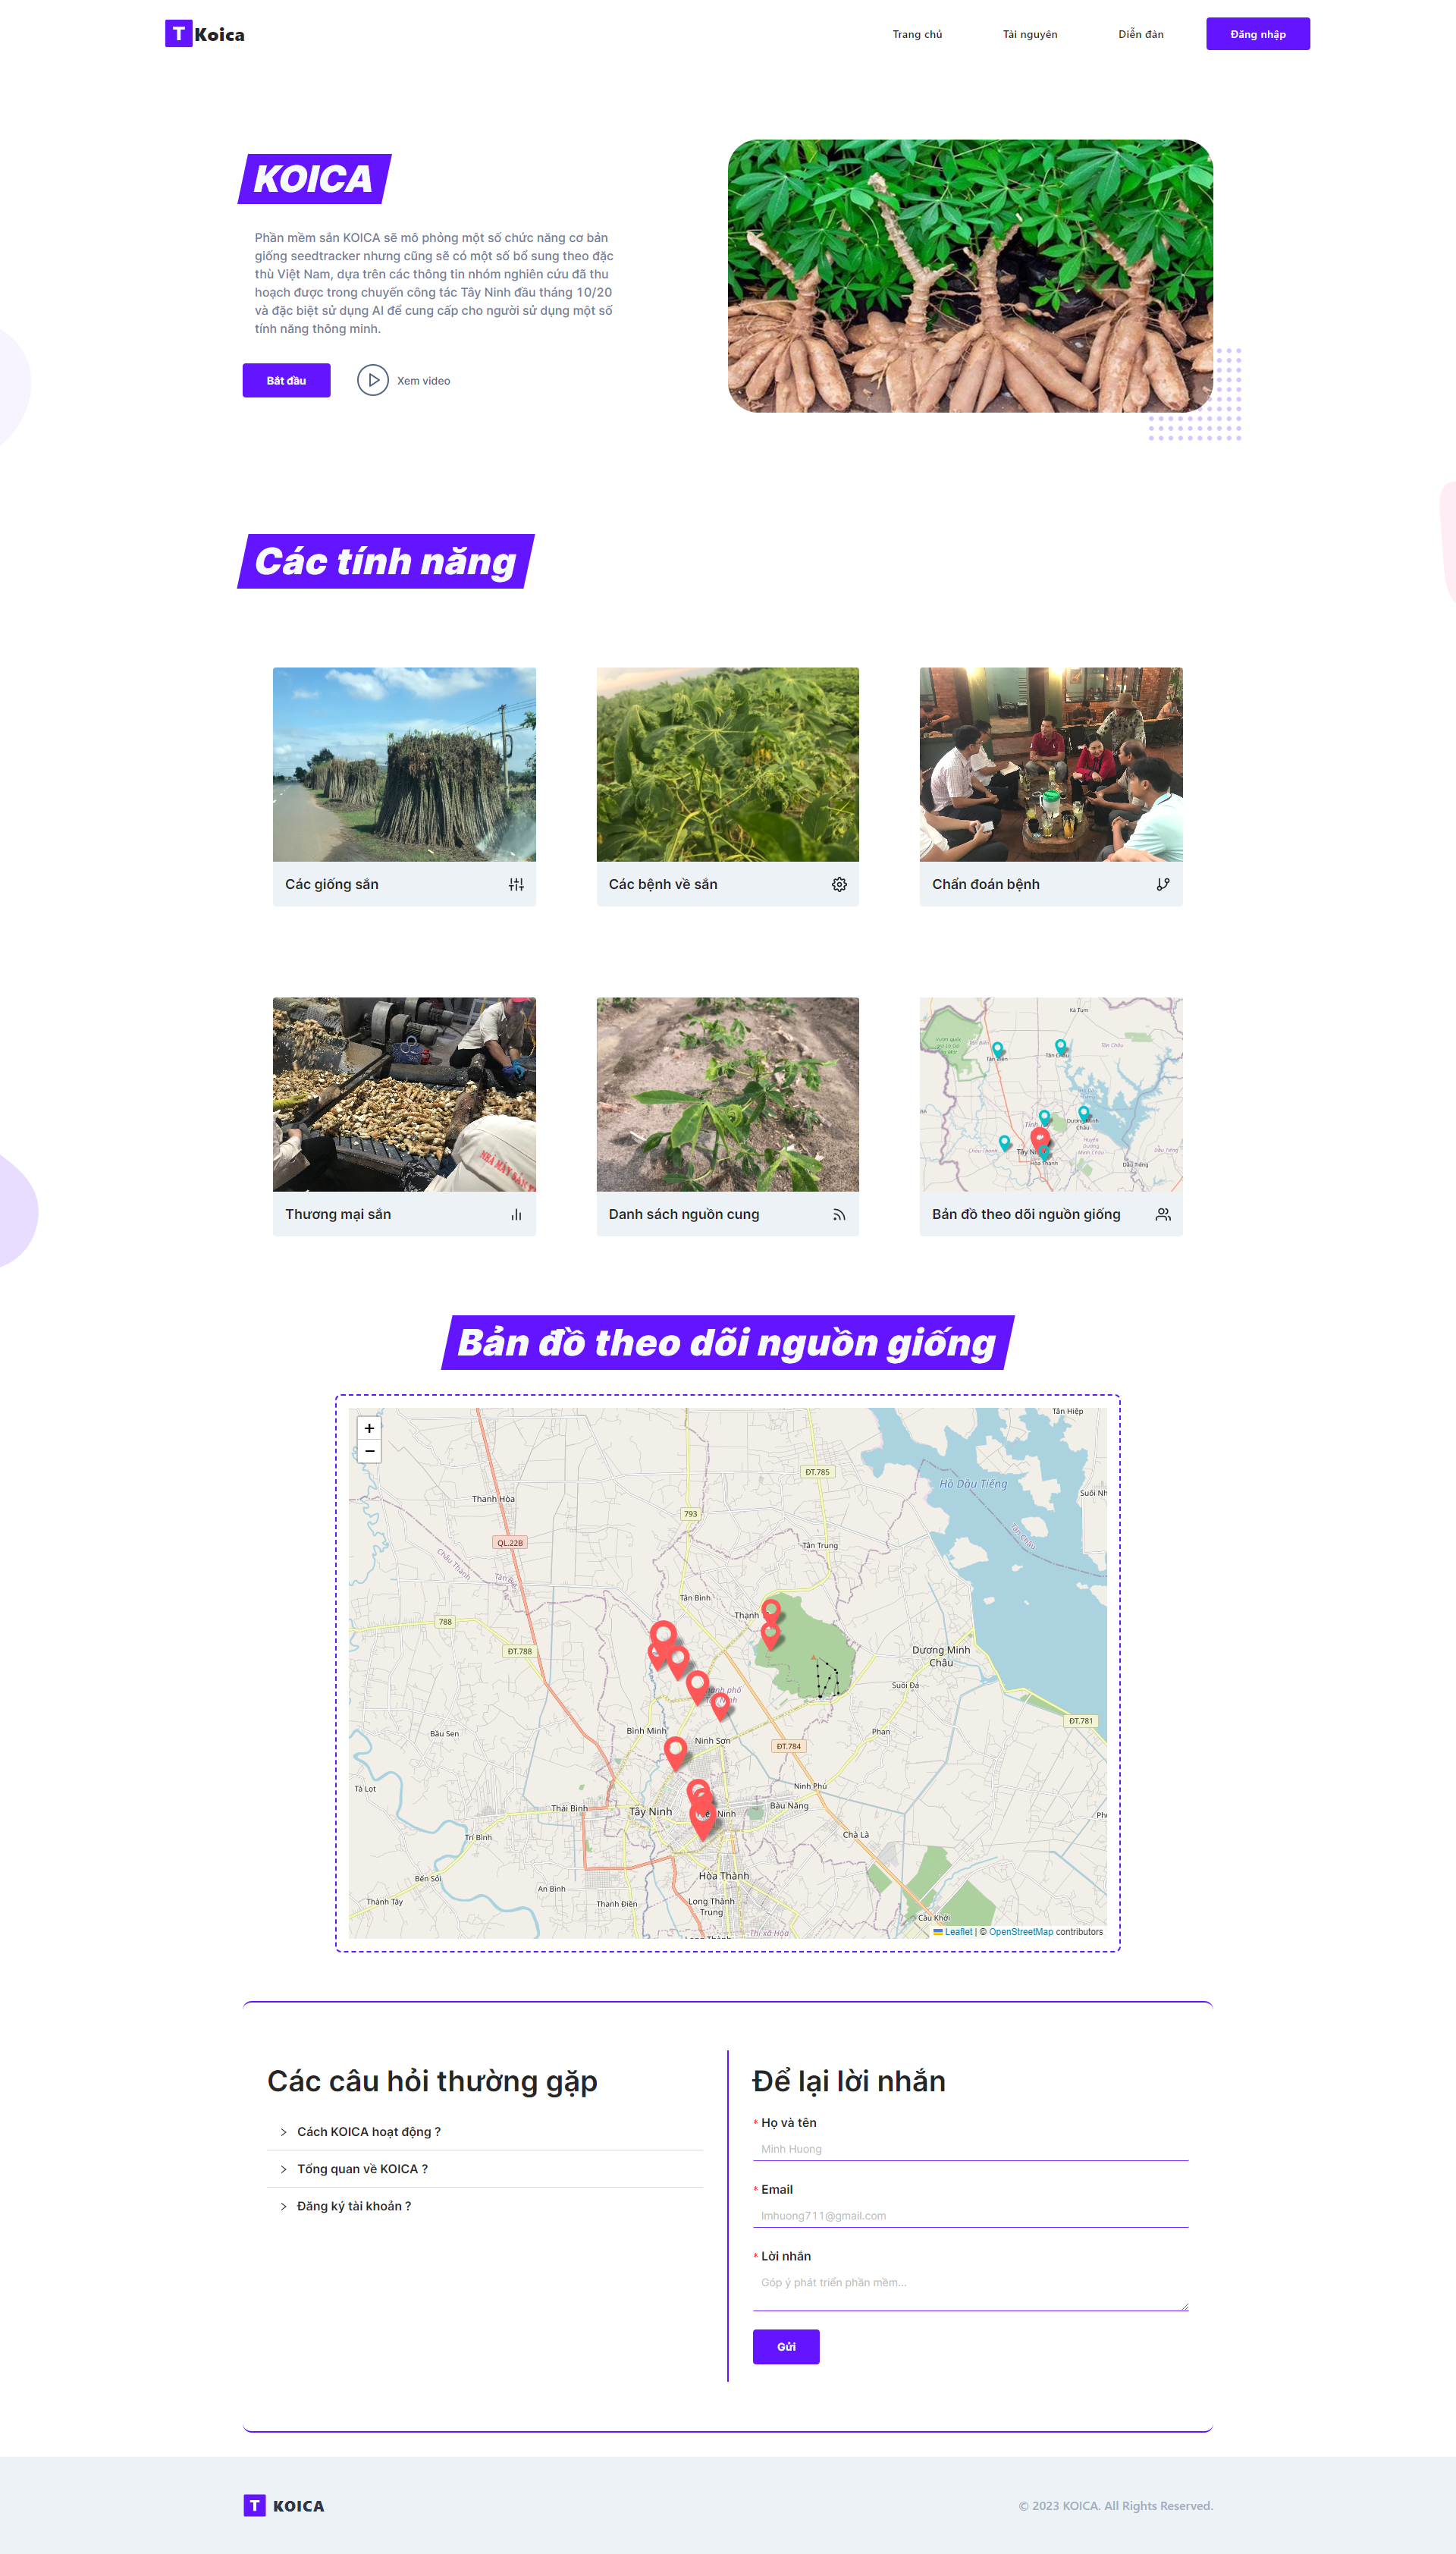
\includegraphics[width=0.95\textwidth,height=0.95\textheight,keepaspectratio]{./img/kltn_homepage.png}
    \caption{Giao diện trang chủ}
    \label{ui:kltn_homepage}
\end{figure}
Hình \ref{ui:kltn_homepage} thể hiện thiết kế giao diện trang chủ của phần mềm. Khi người dùng kéo xuống phần nào, phần mềm sẽ hiển thị giao diện phần tương ứng với các hiệu ứng khi chuyển động trang. Trang chủ được chia làm các phần sau: thanh điều hướng sẽ luôn được hiển thị trên đầu trang, phần giới thiệu phần mềm, phần 6 tính năng chính của hệ thống, phần bản đồ giúp theo dõi dịch bệnh nhanh chóng, phần một số câu hỏi thường gặp và để lại nhận xét, cuối cùng là phần cuối kết thúc trang.

\begin{figure}[H]
\centering
    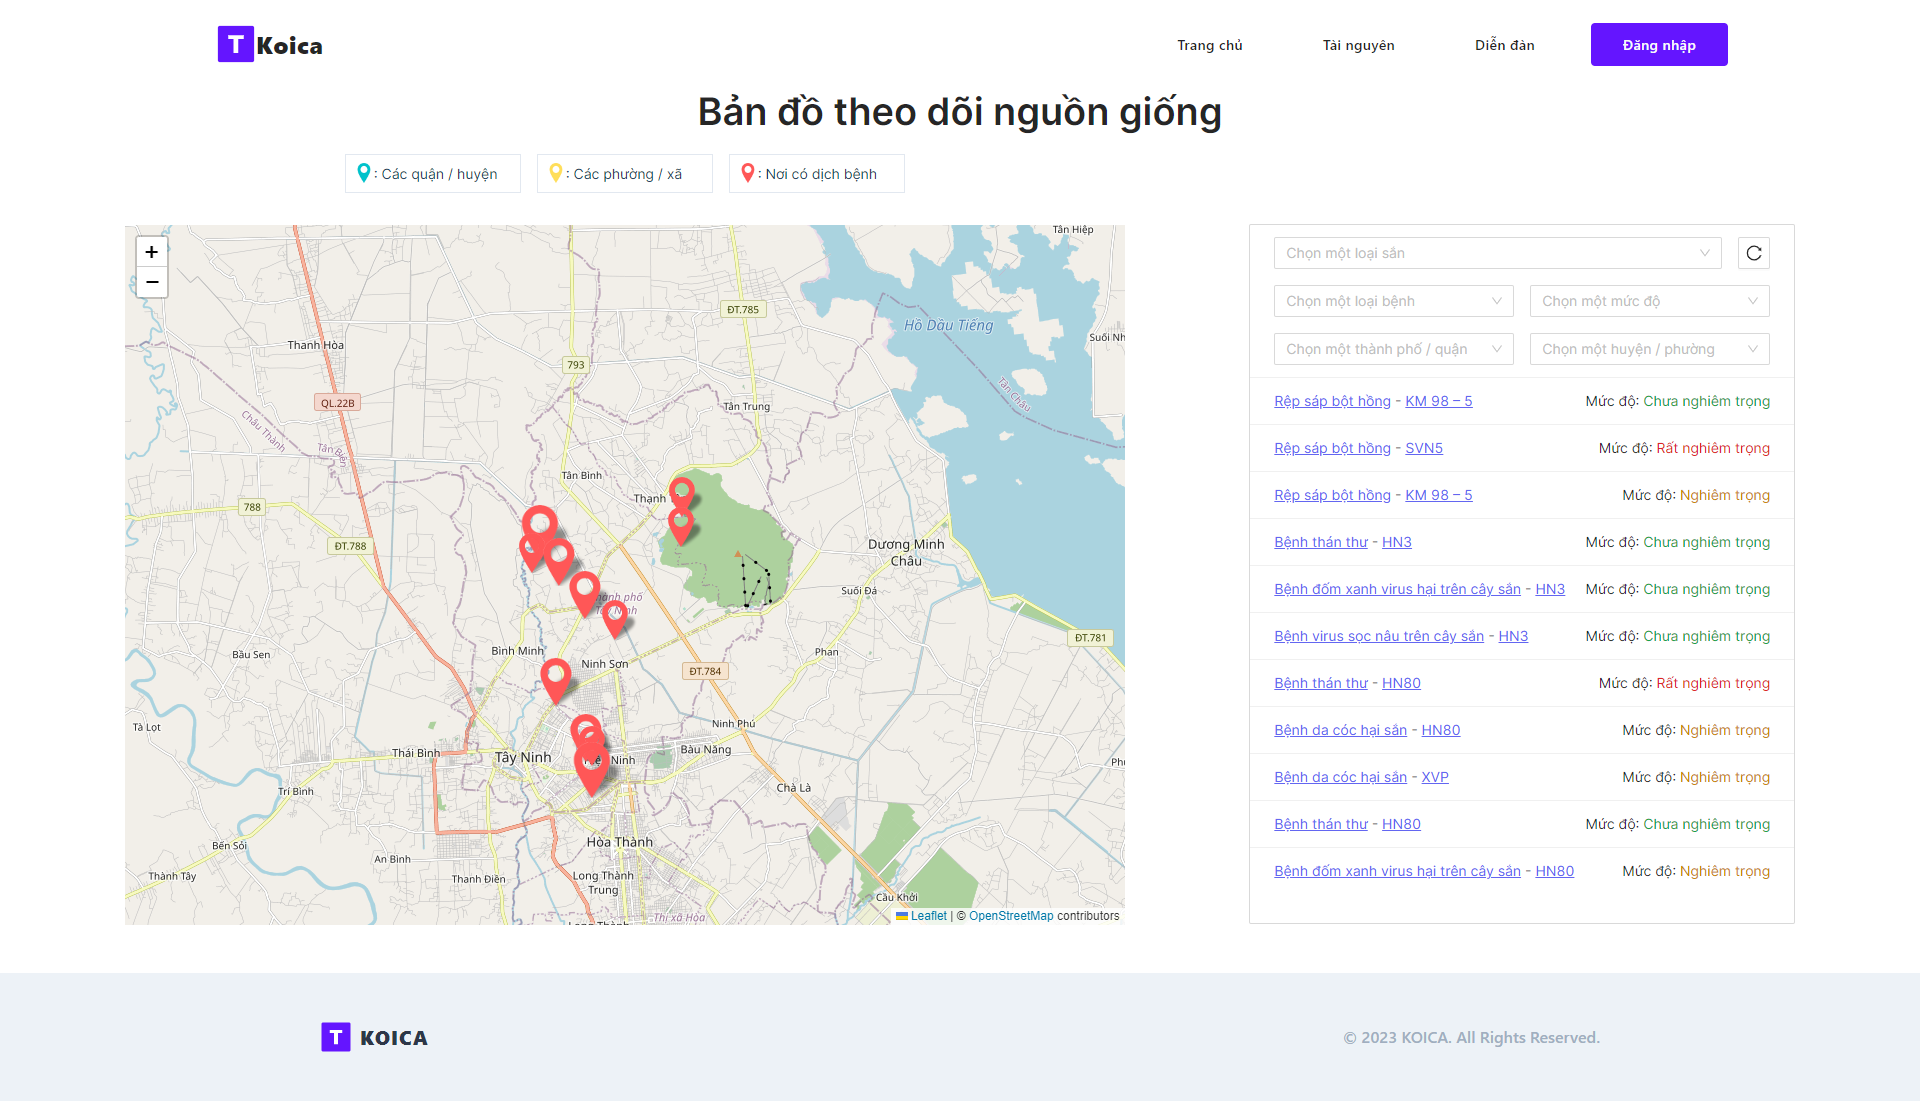
\includegraphics[width=\textwidth,height=\textheight,keepaspectratio]{./img/kltn_map.png}
    \caption{Giao diện màn bản đồ sắn}
    \label{ui:kltn_map}
\end{figure}
Hình \ref{ui:kltn_map} thể hiện thiết kế giao diện bản đồ sắn ở tỉnh Tây Ninh, với các điểm đỏ là nơi diễn ra dịch bệnh, mức độ càng nghiêm trọng thì điểm đỏ càng to. Phía phải giao diện sẽ là bộ lọc dữ liệu giúp người dùng tìm kiếm thông tin dễ dàng hơn.

\begin{figure}[H]
\centering
    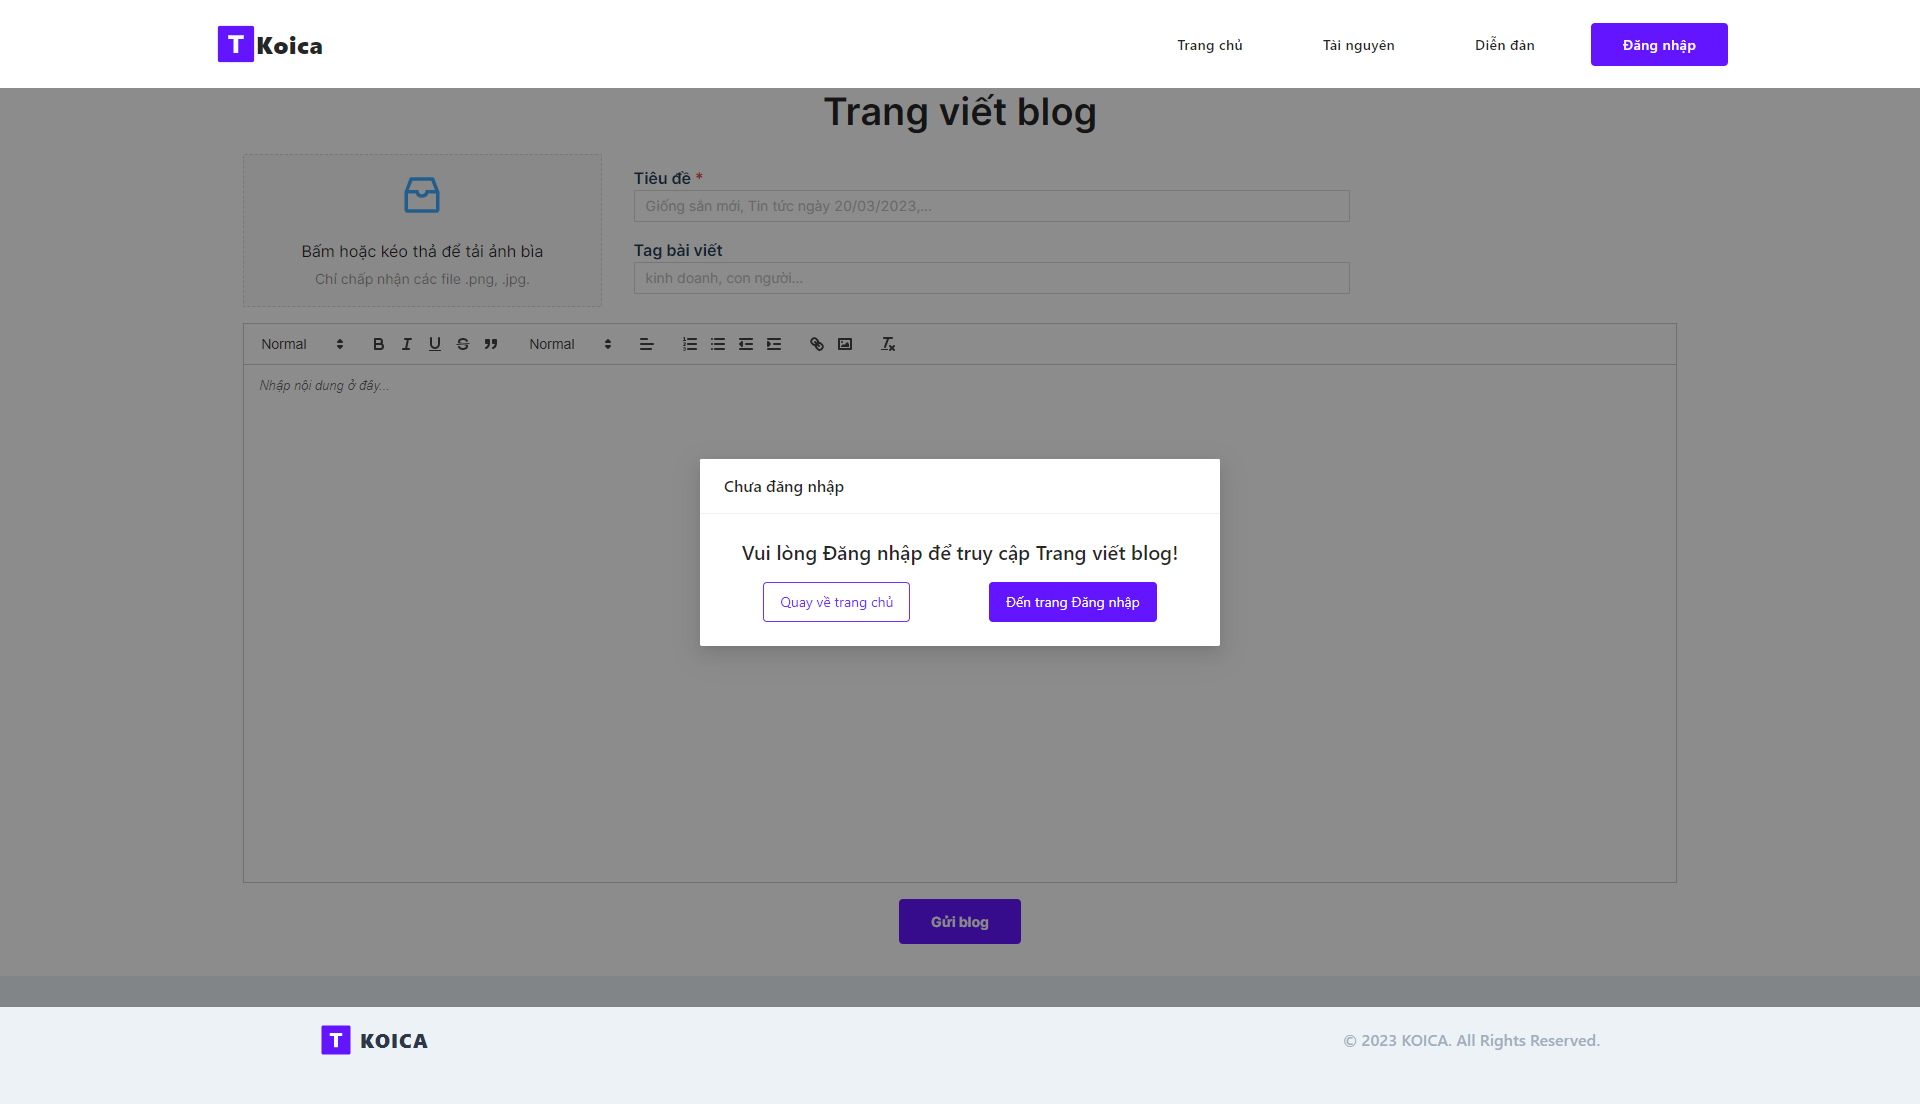
\includegraphics[width=\textwidth,height=\textheight,keepaspectratio]{./img/kltn_guest_createblog.png}
    \caption{Giao diện tạo bài viết mới khi chưa đăng nhập}
    \label{ui:kltn_guest_createblog}
\end{figure}
Hình \ref{ui:kltn_guest_createblog} thể hiện thiết kế giao diện khi người dùng chưa đăng nhập hệ thống mà muốn thực hiện chức năng viết bài. Vì đây là chức năng yêu cầu người dùng phải đăng nhập, nên trang đã hiện thông báo yêu cầu người dùng đăng nhập hoặc quay trở về trang chủ, giới hạn quyền thực hiện các chức năng của tác nhân khách và đảm bảo tính bảo mật.

\begin{figure}[H]
\centering
    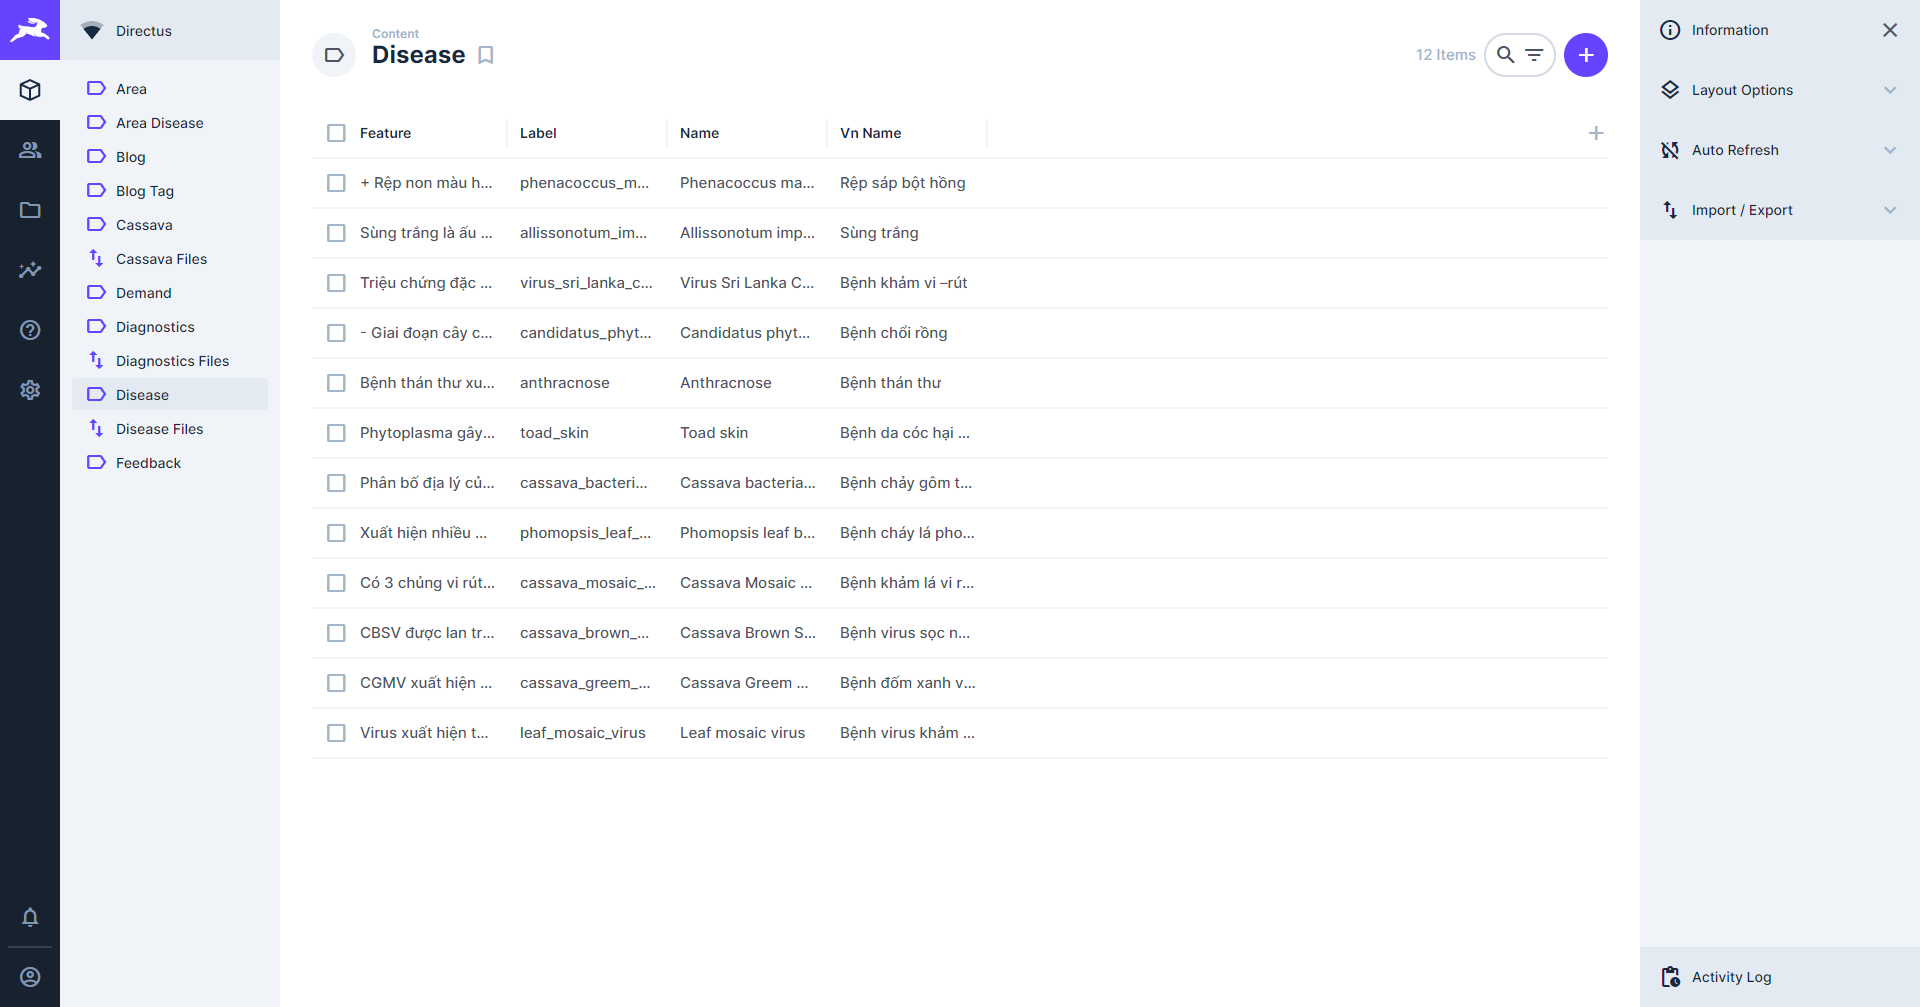
\includegraphics[width=\textwidth,height=\textheight,keepaspectratio]{./img/kltn_be.png}
    \caption{Giao diện quản lý bệnh trên cây sắn ở backend}
    \label{ui:kltn_be}
\end{figure}
Hình \ref{ui:kltn_be} thể hiện thiết kế giao diện ở phía backend. Quản trị viên sau khi đăng nhập có thể thực hiện các thao tác với cơ sở dữ liệu bằng bảng dữ liệu đã được Directus trực quan hóa như hình. Ngoài các bảng dữ liệu được thiết kế thêm, quản trị viên cũng có thể quản lý dữ liệu hệ thống như bảng người dùng, tập chứa các phương tiện truyền thông. Ngoài ra, việc thay đổi kiểu dữ liệu của các trường thông tin, thêm mới bảng dữ liệu, xuất, nhập dữ liệu vào các bảng cũng có thể thực hiện khi có nhu cầu.

\begin{figure}[H]
\centering
    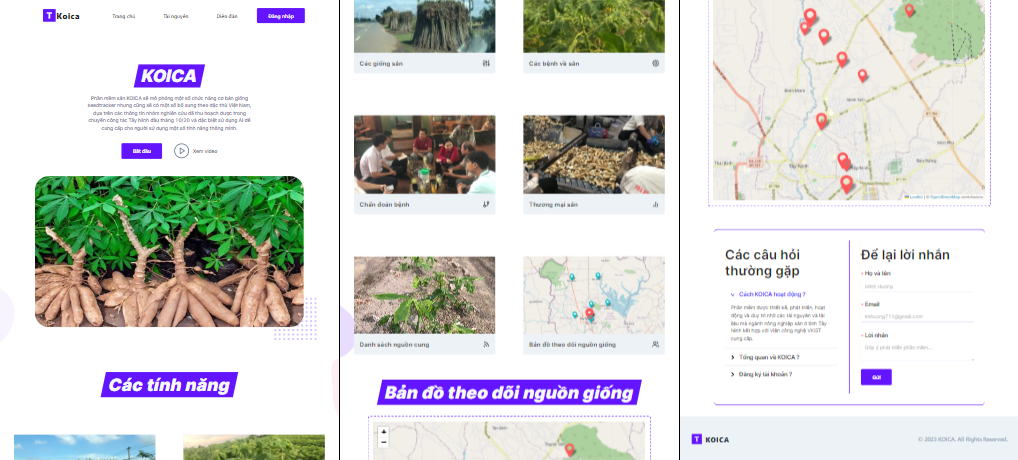
\includegraphics[width=\textwidth,height=\textheight,keepaspectratio]{./img/kltn_responsive.png}
    \caption{Giao diện trang chủ trên máy tính bảng}
    \label{ui:kltn_responsive}
\end{figure}
Hình \ref{ui:kltn_responsive} thể hiện thiết kế giao diện trang chủ trên máy tính bảng thể hiện tính linh hoạt trong bố cục của phần mềm, đảm bảo khả năng tương thích trên nhiều thiết bị người dùng. Ở đây, phần các tính năng chính đã được chia lại thành ba hàng hai cột thay vì hai hàng ba cột như khi xem trên máy tính. Việc này giúp cho trải nghiệm người dùng tốt hơn.

\end{document}
